%% ------------------------------------------------------------------------- %%n
\chapter{Descrição da proposta}
\label{cap:Proposta}

O problema que estamos tratando, classificação de imagens de plâncton, enquadra-se na situação de dados não rotulados abundantes e com elevado custo de rotulação. Conforme mencionado na introdução, o objetivo deste trabalho é o desenvolvimento de métodos para a rotulação e classificação rápida e correta dessas imagens, a fim de que estudos posteriores, dependentes da classificação, tornem-se viáveis. 

Como foi visto no capítulo anterior, o aprendizado ativo é uma possível abordagem para rotular um grande conjunto de amostras, sem requerer a preparação prévia de um conjunto de treinamento grande. Neste processo, o usuário rotula apenas as amostras para as quais o algoritmo solicita um rótulo. De forma geral, o objetivo da abordagem é a minimização do esforço de interação do usuário. O processo continua até que uma boa taxa de classificação seja atingida. Esse classificador pode então ser utilizado para classificar novas amostras. 

Também conforme comentado no capítulo anterior, pesquisas recentes relacionadas à interação de usuários na tarefa de rotulação indicam as limitações do aprendizado ativo clássico. Nesse, o especialista tem uma atuação limitada de apenas confirmar ou corrigir o rótulo atribuído pelo algoritmo a algumas das amostras. Uma forma para contornar essas limitações são abordagens que colocam o especialista em um papel mais central, no qual sua atuação passa a incluir a possibilidade de não só corrigir ou rotular amostras selecionadas pelo algoritmo, mas também participar no processo de seleção das amostras a serem rotuladas \citep{castro2009human, kottke2018other}. Sendo que, no caso dos plânctons, estudos mostram que a incorporação de conhecimentos de especialistas aumenta a acurácia dos modelos \citep{benfield2007rapid}. A figura ~\ref{fig:frameworks_AL} demonstra essa ideia. Do lado esquerdo temos o framework já explicado nos capítulos anteriores, onde o expert participa do processo apenas para aprovar ou desaprovar a classificação feita pelo algoritmo. Do lado direito da figura, temos a mudança na etapa 2, do usuário fazendo parte das escolhas das amostras.

\begin{figure}
  \centering
  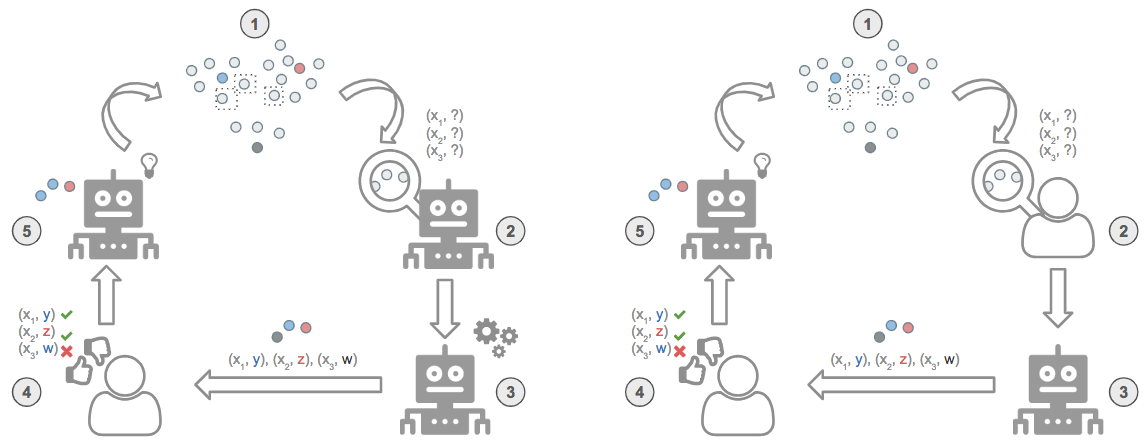
\includegraphics[width=0.9\textwidth]{figures/Frameworks_Active_Learning.png}
  \caption{esq: Framework Aprendizado Ativo Clássico, dir: Framework Aprendizado Ativo com Interação Humana na Seleção de Amostras}
  \label{fig:frameworks_AL}
\end{figure}



A proposta consiste em definirmos formas de interação do usuário, definir formas de usar a informação proveniente dessas interações, e avaliar a efetividade desse uso. Essas etapas estão descritas a seguir. Ao final descrevemos também o conjunto de dados e os procedimentos práticos que serão utilizados na parte experimental do trabalho. 



\section{Estratégia de Interação}
\label{sec:estategia_interacao}

Duas ideias de interação ativa por parte de usuários estão  sendo consideradas nesta proposta. Como elas ainda não estão suficientemente amadurecidas, é possível que a estratégia final seja uma combinação delas.

\subsection{Interação Sobre o Espaço de Projeções}
\label{sec:espaco_projecoes}

Na classificação de imagens, tipicamente são extraídas um conjunto de características das imagens e elas são utilizadas pelos classificadores. No caso de plâncton, características explicitamente extraídas em geral estão relacionados à forma e textura dos organismos. Mais recentemente, com a popularização de redes neurais profundas e, especificamente, das redes convolucionais no caso de imagens, redes pré-treinadas em outros domínios de aplicação podem ser utilizadas como extratores de características. Isto é, dada uma rede pré-treinada, passa-se uma imagem para a rede e extrai-se os valores dessa rede em alguma camada de ativação. O conjunto de valores dessa camada é utilizada como uma representação da imagem de entrada.

Sejam características extraídas explicitamente ou implicitamente, elas podem ser representadas por um vetor em $\mathbb{R}^n$. A visualização de pontos em espaços de dimensão alta não é possível. Portanto, uma técnica comumente utilizada são as projeções desses pontos sobre o espaço 2D.  

Assim como o trabalho de \citep{bernard2018comparing}, as interações dos usuários consistiriam de diferentes formas do usuário interagir com os pontos no espaço 2D.  Deve-se lembrar que cada ponto corresponde a uma imagem. Assim, durante a interação o usuário teria a possibilidade de explorar a estrutura de organização do conjunto de pontos e as imagens associadas a subconjuntos de pontos. Por exemplo, supondo que existam agrupamentos bem definidos na projeção, o usuário poderia inspecionar imagens de um desses agrupamentos e rapidamente determinar a classe predominante no grupo, excluindo apenas as que são de classes distintas. À medida que mais e mais imagens são rotuladas, esses mapas de projeção viriam também acompanhados de cores associados aos pontos já rotulados. Isto poderia ser explorado pelo usuário para rotular amostras em regiões mais críticas (presença de amostras de classes distintas).




\subsection{Interação Sobre Galeria de Imagens} 
\label{sec:galeria_imagens}

Para rotular uma imagem, o especialista precisa ver o organismo presente na imagem. Dado que estamos pressupondo uma representação  das imagens como pontos no $\mathbb{R}^n$, podemos usar métricas de similaridade para selecionar grupos de imagens similares segundo essa métrica e exibir múltiplas imagens de um grupo simultaneamente.
 
Nesta situação, supondo-se que a maior parte dos organismos são de uma mesma classe, em poucas interações o especialista pode corrigir os rótulos errados e confirmar os demais como rótulos corretos. 


\section{Uso das Informações Provenientes da Interação}
\label{sec:uso_das_informacoes_interacao}

A ideia básica do aprendizado ativo de iterar ciclos continua presente. A diferença básica é que o especialista poderá participar de forma mais ativa e selecionar as amostras a serem rotuladas.

A partir da definição de como ocorrerá essa interação, será possível também definir quais tipos de informação estarão disponíveis para o algoritmo gerar um novo classificador melhorado.



\section{Avaliação do método}
\label{sec:avaliação do método}

Propomos neste trabalho avaliar três variações do framework:
\begin{itemize}
    \item {\bf Seleção aleatória de amostras para rotulação}: esta variante é comumente utilizada como baseline quando uma nova estratégia em aprendizado ativo é desenvolvida.
    
    \item {\bf aprendizado ativo clássico}: esta é a variante na qual o oráculo tem um papel passivo de apenas confirmar ou corrigir o rótulo atribuído pelo classificador corrente. Como visto acima, diversas variações são possíveis quanto às estratégias de seleção de amostras para as consultas a serem feitas com o oráculo.
    
\item {\bf Aprendizado ativo com interação ativa de usuário:} este corresponde à variante a ser desenvolvida (oráculo ativo) neste trabalho.
\end{itemize}

O desempenho dos algoritmos é tipicamente ilustrado por meio de um gráfico "número de iterações $\times$  acurácia", que mostra como a acurácia do classificador gerado ao longo das iterações melhora com o número de iterações (exemplos podem ser vistos no capítulo~\ref{cap:Experimentos_Resultados}). O ideal é termos uma curva que atinge alta acurácia logo nas primeiras iterações. Em geral a comparação com a curva referente ao aprendizado baseado em seleção aleatória de dados é empregada para mostrar a efetividade de um algoritmo de aprendizado ativo. Esperamos portanto traçar as três curvas e a expectativa é a de que a curva referente ao aprendizado ativo com interação ativa do usuário atinja alta acurácia com um número menor de iterações.

Em um primeiro momento, as interações serão simuladas, uma vez que dispomos de datasets rotulados. Usaremos os rótulos conhecidos como sendo a resposta do oráculo. No entanto, também pretendemos fazer experimentos com usuários especialistas, como detalhado no capítulo~\ref{cap:Cronogramanotes}.

\section{Considerações sobre a parte experimental}
\label{sec:consideracoes_parte_experimental}


\subsection{Base de dados que poderão ser usados} 
\label{sec:base_usadas}

Neste trabalho teremos três bases de dados disponíveis. As especificações de cada uma estão a seguir.

\textbf{LAPS}

Este dataset foi desenvolvido pelo LAPS\footnote{LAPS: Laboratório de Sistemas Planctônicos (LAPS) do Departamento de Oceanografia Biológica, pertencente ao Instituto Oceanográfico da Universidade de São Paulo (IOUSP)} e contém 5.198 imagens de zooplanctons, divididas em 20 classes.

\textbf{NDSB}

Temos cerca de 30.000 imagens de zooplanctons, divididas em 121 classes, coletadas pelo Centro de Ciências Marinhas Hatfield da Universidade Estadual do Oregon. A fitura ~\ref{fig:ndsb} mostra alguns exemplos das imagens.

\begin{figure}
  \centering
  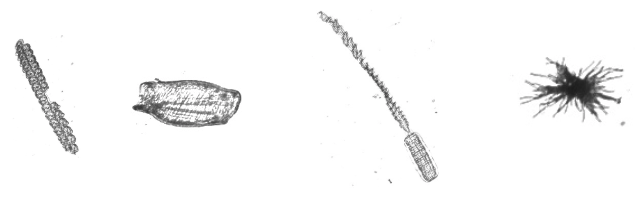
\includegraphics[width=0.9\textwidth]{figures/ndsb_exemplos.png}
  \caption{Exemplos de amostras do dataset NDSB}
  \label{fig:ndsb}
\end{figure}

\textbf{Japan}
Neste dataset temos 32.835 imagens divididas em 23 classes. A figura ~\ref{fig:japan} mostra alguns exemplos das imagens.


\begin{figure}
  \centering
  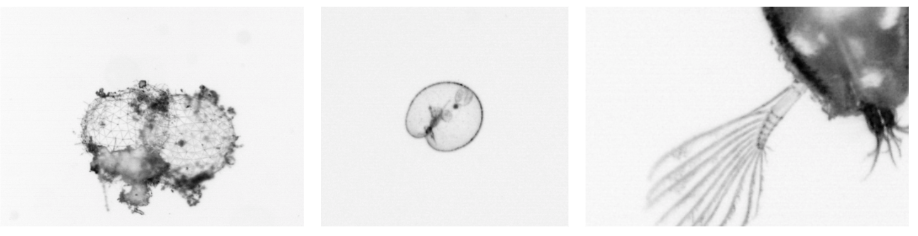
\includegraphics[width=0.9\textwidth]{figures/japan_exemplos.png}
  \caption{Exemplos de amostras do dataset Japan}
  \label{fig:japan}
\end{figure}




%\section{Extração de Features}
%\label{sec:extracao_features}

%A extração de features será feita através de uma arquitetura de Deep Learning. 


%\section{Projeção do Espaço de Features}
%\label{sec:projecao_espaco_features}
